\documentclass[10pt,letterpaper]{article}
\usepackage{spconf,amsmath,amssymb,graphicx,booktabs,url}
\usepackage[T1]{fontenc}
\newcommand{\RCObjective}{0.0834}
\newcommand{\RCSuccess}{89.67}
\newcommand{\RCReductionMyopic}{19.7}
\newcommand{\RCReductionTTL}{11.1}
\newcommand{\RCDiffMyopic}{-0.0204}
\newcommand{\RCLowMyopic}{-0.0249}
\newcommand{\RCHighMyopic}{-0.0161}
\newcommand{\RCDiffTTL}{-0.0104}
\newcommand{\RCLowTTL}{-0.0128}
\newcommand{\RCHighTTL}{-0.0082}
\newcommand{\RCDiffEntropy}{-0.0133}
\newcommand{\RCLowEntropy}{-0.0166}
\newcommand{\RCHighEntropy}{-0.0101}

\title{ReCheck: Task-Sensitive Evidence Refresh Under Hidden Tool Drift}
\name{Author information required before submission}
\address{Controlled-model research draft, 12 September 2026}
\newcommand{\E}{\mathbb{E}}
\newcommand{\ind}{\mathbf{1}}
\begin{document}
\maketitle
\begin{abstract}
A cached tool interpretation can remain syntactically valid after its semantics change. Revalidating every interpretation is expensive, whereas age-only refresh ignores which mistakes matter to the current task. We study evidence refresh as a finite-horizon remote-estimation problem with Markov tasks and hidden binary tool drift. Under independent drift, exact probes and additive loss, the optimal policy factorizes by evidence channel and admits task-dependent age thresholds. This yields ReCheck, an executable reference controller rather than a general language-agent safety guarantee. Across 9,216 controlled trajectory runs, ReCheck reduces weighted loss plus assigned probe cost by \RCReductionMyopic\% relative to myopic refresh and \RCReductionTTL\% relative to development-tuned time-to-live. A separate SQLite experiment executes 5,120 task-method evaluations without changing tool schemas. Unweighted accuracy, model misspecification and runtime measurements expose important limits; no language-model or public-benchmark result is claimed.
\end{abstract}
\begin{keywords}
active sensing, evidence refresh, task-aware estimation, tool drift, agent memory
\end{keywords}

\section{Introduction}
A tool call may retain its name, argument types and output schema while changing an operational convention: an amount may switch units, or a time-range endpoint may become inclusive. An old interpretation can then produce an executable but incorrect result. Refreshing the interpretation before every use avoids this particular failure under a reliable probe, but spends observations even when old evidence remains useful. Never refreshing makes performance depend on unobserved changes. The relevant question is therefore not simply whether a memory is old, but whether obtaining new evidence is worth its cost for present and subsequent decisions.

This problem connects agent memory to task-aware remote estimation. The age of incorrect information distinguishes meaningful estimation error from elapsed time alone \cite{aoii}. Within language-agent research, GLOVE detects memory--environment disagreement and actively re-estimates local responses \cite{glove}. SafeCommit considers alternative latent worlds and gathers evidence before releasing an action \cite{safecommit}. Environment-probing curation checks candidate memories after a task \cite{grounding}, while a recent controlled study shows how scarce verification slots can miss stale decision constraints \cite{stale}. Consequently, active verification, relevance-sensitive probing and memory validation are not new in themselves.

We isolate a narrower question: \emph{how should verified evidence be refreshed across a stream of tasks when its reuse value changes with the task process?} We provide a finite model in which this question can be answered exactly, then use it as a mechanism test. Our contributions are a task-conditioned, factorized refresh recurrence with an explicit threshold argument; a reproducible cost--accuracy study with tuned simple baselines; and an executable SQL transport check with unchanged schemas. The resulting evidence supports a conditional scheduling benefit, not a claim that a new general agent architecture has been validated. A single-task information-gain objective, such as the active-test objectives studied in \cite{ec2}, is an important conceptual neighbor but does not automatically price repeated future reuse.

\section{Problem and information boundary}
There are $d$ evidence channels. Channel $j$ describes a binary tool mode $z_{t,j}\in\{0,1\}$ evolving by independent symmetric flips of probability $h_j\in[0,1/2]$ between tasks. An exact probe costs $c_j>0$, reveals the current mode and resets its evidence age to zero. At startup all methods receive the same exact calibration prefix, and its $d$ probes are charged. A task $k_t\in\{1,\ldots,K\}$ follows an exogenous Markov chain with known transition matrix $P$; it is observed before the refresh decision. The controller knows $P$, the hazards, prices and public task weights $w_{kj}\geq0$, but not current modes, future task realizations or evaluation labels.

The executor uses the most recently observed mode $\widehat z_{t,j}$. This is a maximum-a-posteriori estimate because symmetric drift with $h_j\leq1/2$ does not make the opposite bit more probable. For task $k$, the decision loss is
\begin{equation}
 \ell(k,z,\widehat z)=\sum_{j=1}^{d}w_{kj}\ind\{z_j\ne\widehat z_j\}.
 \label{eq:loss}
\end{equation}
This is an \emph{additive semantic-mismatch loss}, not a guarantee that an arbitrary language model reasons correctly. Exact-task success is a separate diagnostic: every positive-weight channel must be correct. Tasks with zero weights are legitimate negative controls and are counted explicitly.

For a stream of length $T$, the primary objective is
\begin{equation}
 J(\pi)=\frac{1}{T}\E_{\pi}\!\left[\sum_{t=1}^{T}\ell_t+
                  \sum_{u\in\mathcal P_\pi}c_u\right].
 \label{eq:objective}
\end{equation}
$\mathcal P_\pi$ includes startup; $c_u$ is a normalized price. We separately report loop and planning time. There is no common hard probe cap, batch setup charge, observation noise or drift caused by the chosen action. These exclusions are necessary for the following factorization.

\section{Task-conditioned refresh}
\subsection{Belief from evidence age}
After $a$ transitions since an exact observation, the mismatch probability is
\begin{equation}
 p_j(a)=\frac{1-(1-2h_j)^a}{2}.
 \label{eq:parity}
\end{equation}
Indeed, the cached bit is wrong exactly when an odd number of flips occurred. Equivalently, $p_j(a+1)=h_j+(1-2h_j)p_j(a)$ with $p_j(0)=0$. Keeping only age, task and remaining horizon is therefore sufficient in this model. This is a model-based sufficient statistic, not an estimated confidence score from an LLM.

Let $V_{r,j}(a,k)$ be the optimal remaining expected loss and probe cost for channel $j$, with $r$ tasks left. Define $V_{0,j}=0$ and
\begin{align}
 Q^{\rm keep}_{r,j}(a,k)&=w_{kj}p_j(a)
       +\sum_lP_{kl}V_{r-1,j}(a+1,l),\\
 Q^{\rm refresh}_{r,j}(a,k)&=c_j
       +\sum_lP_{kl}V_{r-1,j}(1,l),\\
 V_{r,j}(a,k)&=\min\{Q^{\rm keep}_{r,j},Q^{\rm refresh}_{r,j}\}.
 \label{eq:bellman}
\end{align}
A refreshed channel has zero current mismatch, then age one at the next task. ReCheck refreshes only on a strict improvement, retaining evidence on a tie.

\subsection{Conditional optimality and age thresholds}
\textbf{Proposition 1.} Under the model above, the joint optimal value is $\sum_j V_{r,j}(a_j,k)$. For each fixed $(r,k,j)$, a refresh-optimal region is an upper interval of ages, possibly empty.

\emph{Proof.} At zero remaining horizon, the additive decomposition holds. Suppose it holds for $r-1$. Costs add by channel, task transitions are unaffected by actions, and each channel's next age depends only on its own refresh decision. The joint minimization over the Cartesian product of binary refresh actions therefore equals the sum of channelwise minima in (\ref{eq:bellman}). For monotonicity, $p_j(a)$ is nondecreasing. If $V_{r-1,j}(a,l)$ is nondecreasing for every $l$, then $Q^{\rm keep}$ is nondecreasing in age and $Q^{\rm refresh}$ is constant. Their minimum is nondecreasing, and once refresh is strictly better it remains so. Induction completes the argument. $\square$

This specializes standard dynamic programming, not a general theorem for memory. A finite table over reachable ages has $O(T^2Kd)$ entries and $O(T^2K^2d)$ arithmetic cost with a dense task transition matrix. Values can be computed offline for each declared model; runtime selection uses $d$ table lookups. Stored policy tables remain model-specific and must be rebuilt if the model changes.

\subsection{Why present-task myopia can fail}
Myopic refresh compares only $w_{kj}p_j(a)$ with $c_j$. Consider two remaining tasks, hazard $0.05$, price $0.12$, age five and weights $0.35$ then $0.65$. The current risk is $0.0717<0.12$, so myopic refresh waits. At the next task, refreshing costs $0.12$, giving total expected cost $0.1917$. Refreshing now costs $0.12+0.65(0.05)=0.1525$: the observation is useful twice. This hand-computable case, also checked by a unit test, explains how reuse can justify a refresh that current risk alone rejects.

The model does not justify every form of proactive probing. With independent channels and no shared budget, it does not generally reward inspecting an entirely irrelevant channel just to accumulate facts. Nor does channelwise optimization capture complementary observations. For a uniformly unknown two-bit XOR decision, one exact bit conveys no answer information, whereas both bits do. At price $0.1$ per bit, no probe costs $0.5$ expected error, one costs $0.6$, and both cost $0.2$. This diagnostic is outside the additive theorem and is not counted as a ReCheck success.

\section{Executed study}
\subsection{Protocol and comparisons}
We use four channels and six task rows,
\begin{equation}
 W=\begin{bmatrix}
1&0&0&0\\0&.35&0&0\\0&0&.65&0\\0&0&0&.2\\
.6&.15&.25&0\\0&0&0&0
\end{bmatrix}.
\end{equation}
Tasks follow
\begin{equation}
 P=\rho I+(1-\rho)\mathbf{1}\mathbf{1}^{\top}/6,\qquad \rho\in\{0.2,0.9\}.
\end{equation} Channel hazards use multipliers $(0.5,1,1.5,0.8)$ with base rates $0.01$, $0.05$ and $0.15$; probe prices are $0.04$, $0.12$ or $0.35$. Each trajectory contains 80 tasks. The same 64 test seeds generate paired realizations for eight policies across all 18 configurations, giving 9,216 runs and 737,280 task-method evaluations. These are generator replications, not unseen-task-family generalization.

Baselines are never refresh, fresh relevant channels, time-to-live (TTL), a mismatch-probability threshold, random relevant refresh, and myopic decision-cost refresh. TTL, probability thresholds and random probabilities are selected separately per configuration on 16 disjoint development seeds. The no-task ablation replaces each task's weights by their marginal mean but keeps the same dynamic-programming implementation. All policies have the same mode hypotheses and probe access. None is labeled a faithful reproduction of GLOVE or SafeCommit; their different interfaces and full agent mechanisms were not run.

Before the main execution, configuration and source hashes were frozen locally. This was not external preregistration. Sanity inspection revealed that common seeds couple regimes; the documented analysis amendment therefore clusters \emph{all} regimes and prices by the 64 base seeds rather than pretending there are 384 independent streams. Reported intervals use 3,000 paired cluster bootstrap replicates and are descriptive, with no familywise significance claim.

\begin{table}[t]
\centering
\caption{Controlled main study. Probes include startup and are per task. Success is unweighted; loss is (\ref{eq:loss}).}
\label{tab:main}
{\fontsize{9}{11}\selectfont\setlength{\tabcolsep}{3pt}\begin{tabular}{lrrrr}
\toprule
Policy & Success (\%) & Loss & Probes & $J$ \\
\midrule
Never & 62.27 & 0.1988 & 0.050 & 0.2073 \\
Fresh & 100.00 & 0.0000 & 1.210 & 0.2057 \\
Tuned TTL & 89.60 & 0.0473 & 0.437 & 0.0938 \\
Mismatch threshold & 91.93 & 0.0393 & 0.479 & 0.0966 \\
Random & 88.23 & 0.0537 & 0.567 & 0.1128 \\
Myopic & 80.68 & 0.0760 & 0.325 & 0.1038 \\
No task weights & 81.73 & 0.0705 & 0.515 & 0.1197 \\
ReCheck & 89.67 & 0.0339 & 0.443 & 0.0834 \\
\bottomrule
\end{tabular}}
\end{table}

\subsection{Weighted objective versus accuracy}
Table~\ref{tab:main} reports mean realized costs. ReCheck attains $J=\RCObjective$, a \RCReductionMyopic\% reduction relative to myopic refresh and \RCReductionTTL\% relative to tuned TTL. Paired differences are \RCDiffMyopic\ [\RCLowMyopic,\RCHighMyopic] and \RCDiffTTL\ [\RCLowTTL,\RCHighTTL], respectively. The mismatch-threshold difference is \RCDiffEntropy\ [\RCLowEntropy,\RCHighEntropy]. These intervals quantify variation over the generator, not uncertainty about deployment distributions.

ReCheck's exact-task success is \RCSuccess\%, below the mismatch-threshold baseline's 91.93\%. Fresh achieves 100\% under exact probes, at a much larger probe bill. Thus optimizing severity-weighted loss does not guarantee the best unweighted accuracy. Figure~\ref{fig:frontier} shows the close success--probe trade-offs; it does not support dominance over every operating point. Figure~\ref{fig:drift} shows how the weighted objective changes with hazard. The no-task ablation's $J=0.1197$ further indicates that the scheduler needs the task weights, not only evidence age.

\begin{figure}[t]
\centering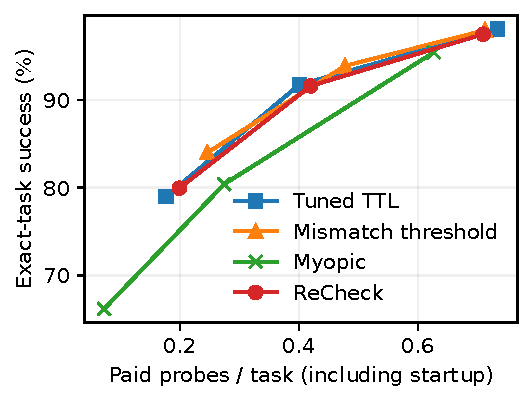
\includegraphics[width=\columnwidth]{figures/recheck_frontier.pdf}
\caption{Three price settings per curve, pooled across drift and task persistence. Mismatch thresholds can achieve higher unweighted success; the optimized objective also weights error severity.}
\label{fig:frontier}
\end{figure}

\begin{figure}[t]
\centering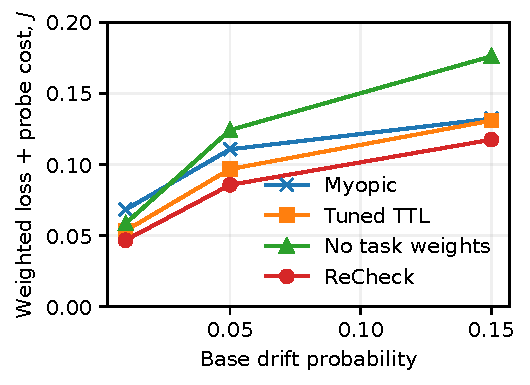
\includegraphics[width=\columnwidth]{figures/recheck_drift.pdf}
\caption{Realized weighted objective by base hazard, averaged over both task-persistence settings and all prices.}
\label{fig:drift}
\end{figure}

\subsection{Executable SQL transport}
A separate adapter changes amount encoding and interval endpoint semantics in an in-memory SQLite database while preserving table schemas. Probes execute actual SQL on calibration records and a boundary marker. Amount, count, combined and irrelevant-schema tasks are performed by a deterministic interpreter, not a language model. Thirty-two new seeds, 40 tasks and four policies yield 5,120 executed task-method evaluations. Every schema-fingerprint check passes.

\begin{table}[t]
\centering
\caption{SQLite experiment; the source data and drift are synthetic, but SQL calls and returned task results are executed.}
\label{tab:sql}
{\fontsize{9}{11}\selectfont\setlength{\tabcolsep}{4pt}\begin{tabular}{lrrr}
\toprule
Policy & Success (\%) & Probes & $J$ \\
\midrule
Never & 73.44 & 0.050 & 0.2376 \\
Fresh & 100.00 & 0.972 & 0.1166 \\
Myopic & 88.52 & 0.232 & 0.1091 \\
ReCheck & 95.62 & 0.376 & 0.0756 \\
\bottomrule
\end{tabular}}
\end{table}

ReCheck improves success over myopic refresh by 7.11 percentage points [3.91,10.78], with objective difference $-0.0335$ [$-0.0586,-0.0115$]. It remains below fresh on success by 4.38 points. Mean task-loop time is 3.17\,ms per 40-task stream versus 2.62\,ms for myopic refresh; these times exclude shared setup, startup calibration and policy compilation. The observation-cost objective must not be presented as measured end-to-end speed or monetary savings. Compilation timings and complete per-run ledgers are retained in the artifact.

\subsection{Boundary checks}
With zero drift and exact startup, never, myopic and ReCheck all achieve 100\% success and $J=0.006$, the startup cost only. When the true base hazard is $0.15$ but the controller assumes $0.01$, ReCheck's $J$ rises to $0.1421$, worse than fresh's $0.1365$. When hazard is overestimated, ReCheck spends more observations and its $J=0.0698$ exceeds myopic's $0.0625$. These are explicit failures of model calibration, not anomalies removed from the main table. A noisy binary Bayes update is unit-tested, but the main controller and measurements assume exact probes; noisy-observation robustness has not been established.

\section{Scope, limitations and conclusion}
The strongest result is conditional: task-dependent future reuse improves a known-model evidence-refresh objective. It rests on supplied task dependencies, known transition and drift probabilities, correct startup evidence, separable costs and exact probes. It does not establish dependency extraction, unknown-hazard learning, hard-budget coordination, open-world candidate coverage or natural-language reasoning reliability. There are no real LLM calls, public benchmark scores, external-domain generalization tests or independently audited human labels in this study. Small known-model scheduling is a reference experiment, not sufficient evidence of a complete deployed agent.

The accompanying code contains unit and exhaustive small-case checks, raw paired trajectories, SQL receipts, frozen source hashes and generated tables. All reported measurements come from execution. The practical next test is to estimate hazards and dependencies on separate development environments, then compare a full agent under total measured cost. Until that test, the defensible contribution is an exact task-sensitive model, a reproducible scheduling benefit, and its documented boundaries.

\section{Acknowledgments and AI disclosure}
ChatGPT (OpenAI) assisted with method formulation, code, plotting code and text in all sections. Tables and figures were generated from executed experiments. No independent human validation is claimed. This draft requires responsible human authorship and review before submission.

\begin{thebibliography}{9}
\bibitem{aoii} A.~Maatouk, M.~Assaad, and A.~Ephremides, ``The age of incorrect information: An enabler of semantics-empowered communication,'' arXiv:2012.13214, 2020, revised 2022.
\bibitem{glove} X.~Yin and H.~Du, ``GLOVE: Global verifier for LLM memory-environment realignment,'' arXiv:2601.19249, 2026.
\bibitem{safecommit} M.~Akewar and R.~Ranjan, ``SafeCommit: Certifying when memory-grounded agents may safely act,'' arXiv:2608.04289, 2026.
\bibitem{grounding} S.~Suresh, H.~Mak, S.~Bhatnagar, C.~Methani, and A.~Gutierrez Munoz, ``Grounding agent memory: Environment-probing curation for enterprise agents,'' arXiv:2609.11060, 2026.
\bibitem{stale} K.~Nakayashiki, ``When stale constraints go unchecked: Budgeted verification failures in inherited agent memory,'' arXiv:2608.25553, 2026.
\bibitem{ec2} D.~Golovin, A.~Krause, and D.~Ray, ``Near-optimal Bayesian active learning with noisy observations,'' in \emph{Advances in Neural Information Processing Systems}, vol.~23, 2010, pp.~766--774.
\end{thebibliography}
\end{document}
